\documentclass[11pt, a4paper]{article}
\usepackage[margin=2.2cm]{geometry}
\usepackage{booktabs}
\usepackage{graphicx}
\usepackage{parskip}
\usepackage{hyperref}
\usepackage{caption}
\graphicspath{{figures/}}

\title{\textbf{Phase 1 Report — Clustering Analysis on DS-10}}
\author{Advanced Data Mining, Spring 1404--1405}
\date{\today}

\begin{document}
\maketitle

\section{Introduction}
DS-10 is the UCI/Kaggle Credit Card Fraud dataset: 284{,}807 transactions with 28 PCA-anonymised numeric features (V1--V28), a \texttt{Time} offset (seconds from the first transaction), a transaction \texttt{Amount}, and a binary \texttt{Class} label (492 fraudulent). The central clustering research question is whether transactions form density-distinct subpopulations that separate fraudulent from legitimate behaviour --- recoverable without using the label. Labels are used only as external evaluation in Phase 2.

\section{Ingestion and schema}
A pandera schema (\texttt{src/clustering\_analysis/schemas.py::RawSchema}) enforces 31 columns, \texttt{Class}~$\in \{0,1\}$, and non-negative \texttt{Amount}/\texttt{Time}. Ingestion produces \texttt{data/raw/manifest.json} recording source URL, SHA-256 checksum, row count, and timestamp. The recorded checksum is \texttt{76274b691b16a6c4\ldots} (full hash in the manifest).

\section{Cleaning decision log}
Exact-duplicate rows dropped: 1{,}081 duplicates removed, leaving 283{,}726 rows for downstream stages. No missing values observed; \texttt{Class} retained but never input to any fitting step. Full per-column rationale lives in the auto-generated \texttt{reports/decision\_log.md}.

\section{Feature engineering}
Three derived features replace the raw \texttt{Time} and \texttt{Amount}: \texttt{log\_amount}~$= \log(1 + \mathrm{Amount})$ to correct heavy right skew, and \texttt{time\_sin}, \texttt{time\_cos} encoding \texttt{Time}~$\bmod\ 86400$ as a unit-circle phase. V1--V28 pass through unchanged (already PCA from source). The delivered feature set has 31 columns.

\section{Scaling}
Three strategies compared (Strategy A: uniform Standard; B: uniform Robust; C: hybrid). Strategy~C is selected: \texttt{StandardScaler} on V1--V28 (already roughly $\mathcal{N}(0,1)$) and \texttt{RobustScaler} on \texttt{log\_amount} + cyclic time. Figure~\ref{fig:scaling} shows the V1$\times$V14 scatter under each strategy.

\begin{figure}[h]\centering\includegraphics[width=0.7\linewidth]{scaling_comparison.pdf}
\caption{Scaling strategy comparison (Phase 1 \S4.5).}\label{fig:scaling}\end{figure}

\section{Dimensionality reduction}
PCA at 95\% cumulative variance retains 28 components (Fig.~\ref{fig:pca}). UMAP (\texttt{n\_neighbors=30}, \texttt{min\_dist=0.05}) provides the 2D density view (Fig.~\ref{fig:umap}) and a 10D embedding held for Phase 2 density-based methods.

\begin{figure}[h]\centering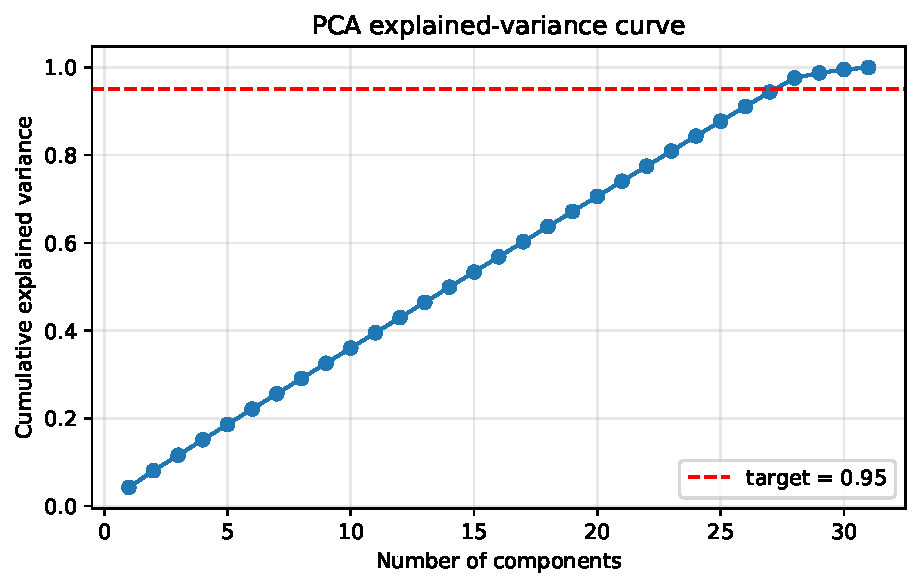
\includegraphics[width=0.7\linewidth]{pca_explained_variance.pdf}
\caption{PCA cumulative explained variance.}\label{fig:pca}\end{figure}
\begin{figure}[h]\centering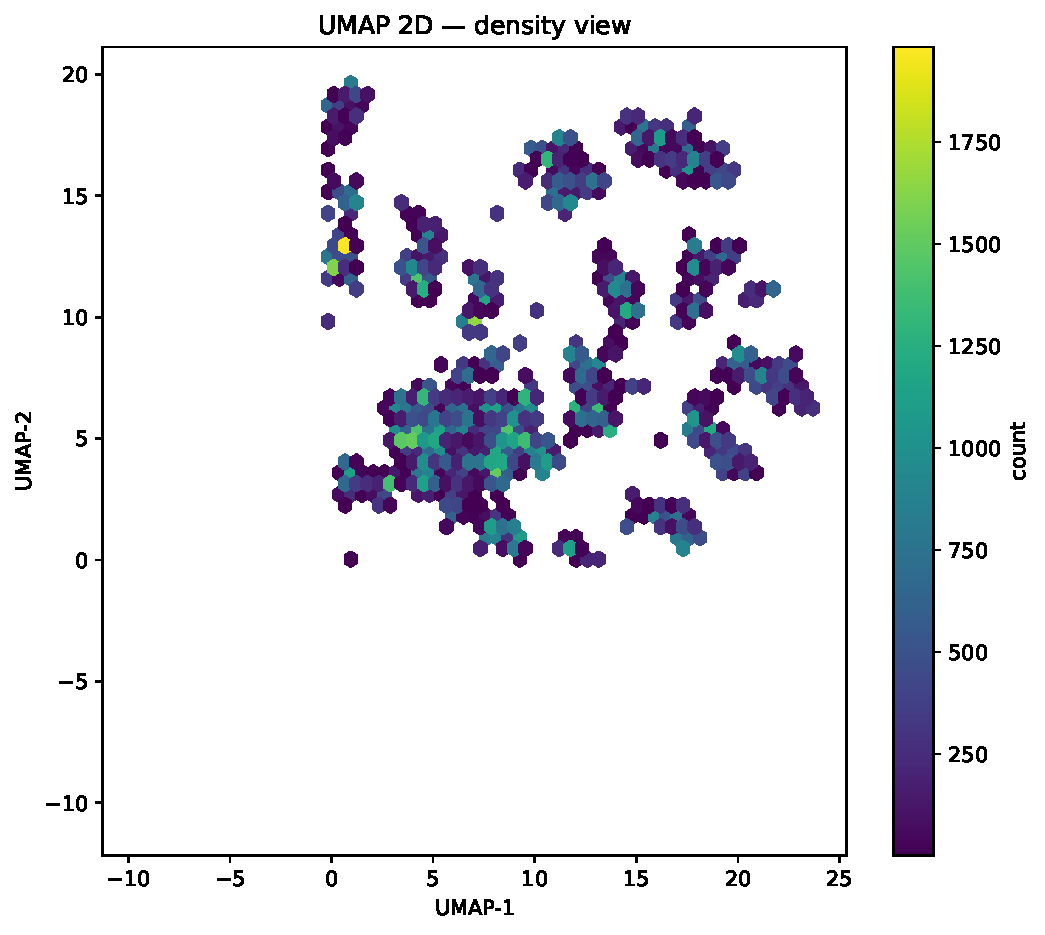
\includegraphics[width=0.7\linewidth]{umap_density.pdf}
\caption{UMAP 2D density (hexbin) — qualitative cluster structure.}\label{fig:umap}\end{figure}

\section{Distance metric}
Euclidean ($\ell_2$) is the headline metric for K-Means, Ward, GMM, and HDBSCAN: V-features are PCA-rotated and roughly homogeneous post-scaling. Mahalanobis and cosine are reserved for Phase 2 ablations.

\section{Clustering tendency}
Hopkins~$H$ on the standardised matrix, averaged over 5 seeded repeats, is $H = 1.000 \pm 0.000$; the project's pass threshold is $H \ge 0.6$, so the dataset proceeds to Phase 2. The very high $H$ reflects strong cluster tendency: fraud micro-clusters and the dense legitimate bulk produce nearest-neighbour distances far smaller than uniform-random references in the 31-dimensional space. The VAT heatmap (Fig.~\ref{fig:vat}) on a stratified subsample (2{,}000 legitimate + 492 fraud) surfaces diagonal block structure as qualitative confirmation.

\begin{figure}[h]\centering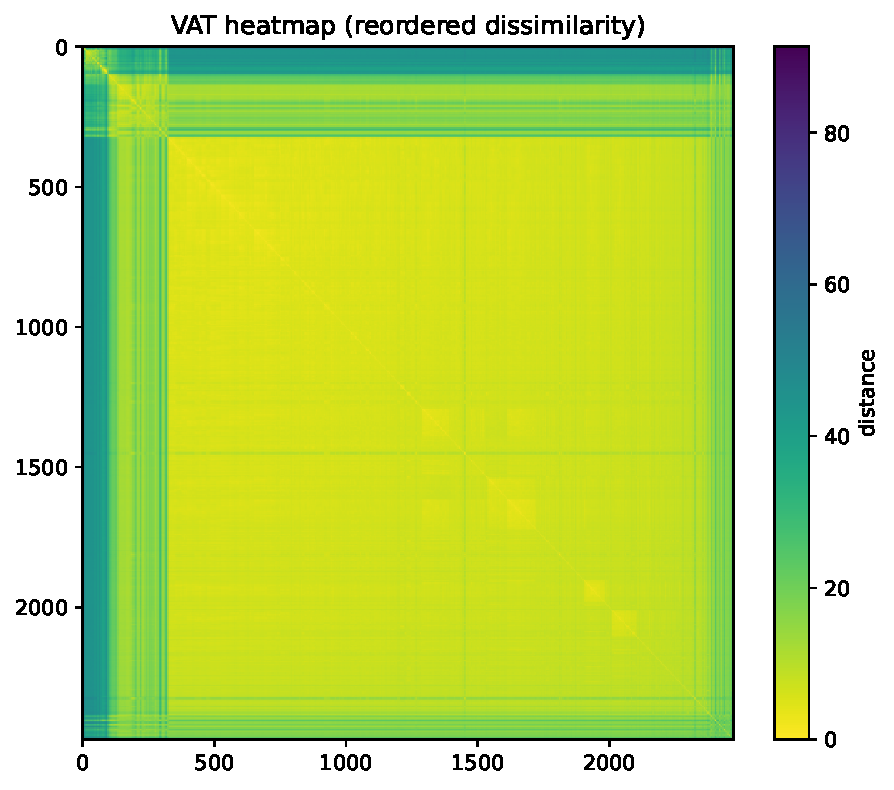
\includegraphics[width=0.55\linewidth]{vat_heatmap.pdf}
\caption{VAT heatmap on stratified subsample.}\label{fig:vat}\end{figure}

\section{Conclusions and hand-off to Phase 2}
Phase 1 outputs (\texttt{X\_scaled}, \texttt{X\_pca}, \texttt{umap\_2d}, \texttt{labels}) are persisted under \texttt{data/processed/}. The Hopkins value strongly supports proceeding with the planned Phase 2 portfolio covering both convex (K-Means, GMM) and density-varying (HDBSCAN, OPTICS) regimes.

\section{Reproduction}
\texttt{make phase1} from a fresh clone with \texttt{data/raw/creditcard.csv} present.

\end{document}
